\documentclass[12pt]{article}

\usepackage[a4paper,margin=1in]{geometry}
\usepackage{amsmath}
\usepackage{amssymb}
\usepackage{enumitem}
\usepackage{tikz}
\usetikzlibrary{
    arrows.meta,
    calc,
    angles,
    quotes,
    decorations.pathmorphing
}
\usepackage[american]{circuitikz}


\setlist[enumerate]{itemsep=1.8em}

\begin{document}

\begin{center}
\Large \textbf{PAPER 7 — Elimination Round Depth}
\end{center}

\begin{enumerate}

\item An incompressible non-viscous liquid flows steadily in a horizontal pipe. At some section, the cross-sectional area decreases by 2\% over a short smooth region, and density remains constant. Using continuity and Bernoulli simultaneously, neglecting terms beyond first order in small changes, determine the approximate fractional change in static pressure at that section relative to upstream pressure.

% =========================
% Diagram for Question 1
% =========================
\begin{center}
\textbf{Diagram for Question 1}
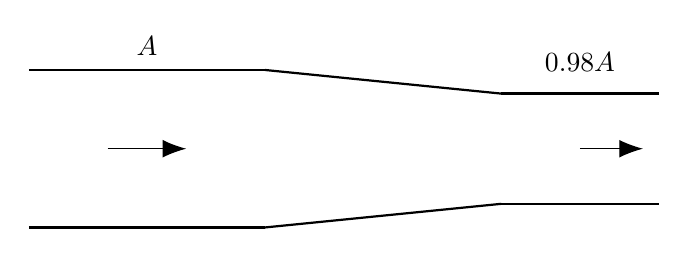
\begin{tikzpicture}[scale=1]
% Pipe narrowing
\draw[thick] (-4,1) -- (-1,1);
\draw[thick] (-4,-1) -- (-1,-1);

\draw[thick] (-1,1) -- (2,0.7);
\draw[thick] (-1,-1) -- (2,-0.7);

\draw[thick] (2,0.7) -- (4,0.7);
\draw[thick] (2,-0.7) -- (4,-0.7);

% Flow arrows
\draw[-{Latex[length=3mm]}] (-3,0) -- (-2,0);
\draw[-{Latex[length=3mm]}] (3,0) -- (3.8,0);

\node at (-2.5,1.3) {$A$};
\node at (3,1.1) {$0.98A$};
\end{tikzpicture}
\end{center}

A) $-4\%$ \\
B) $-2\%$ \\
C) $+2\%$ \\
D) $+4\%$

\item A water jet of cross-section $A$ and speed $v$ strikes a smooth vertical wall and rebounds elastically with unchanged speed. Now the supply pressure is altered so that speed increases by 2\% while the nozzle area decreases by 1\%. Neglecting higher-order terms, determine the approximate fractional change in force exerted on the wall.

% =========================
% Diagram for Question 2
% =========================
\begin{center}
\textbf{Diagram for Question 2}
\begin{tikzpicture}[scale=1]
% Wall
\draw[thick] (3,-2) -- (3,2);

% Jet
\draw[thick,->] (-3,0) -- (3,0);
\draw[thick,->] (2.9,0) -- (-1,0);

\node at (-2,0.5) {$v$};
\node at (0,-0.6) {$A$};
\node at (3.5,1.5) {Wall};
\end{tikzpicture}
\end{center}

A) $1\%$ \\
B) $2\%$ \\
C) $3\%$ \\
D) $4\%$

\item Terminal velocity of a small sphere in a viscous fluid is governed by Stokes’ law. Suppose its radius increases by 5\%, viscosity increases by 3\%, and density difference between sphere and fluid decreases by 2\%, all simultaneously. Ignoring higher-order products of small quantities, estimate the fractional change in terminal velocity.

A) $5\%$ \\
B) $6\%$ \\
C) $4\%$ \\
D) $3\%$

\item Capillary rise is given by $h=\dfrac{2\gamma \cos\theta}{\rho g r}$. If surface tension decreases by 3\% and contact angle changes such that $\cos\theta$ decreases by 2\% while tube radius increases by 1\%, determine the approximate fractional change in capillary rise, neglecting second-order terms.

% =========================
% Diagram for Question 4
% =========================
\begin{center}
\textbf{Diagram for Question 4}
\begin{tikzpicture}[scale=1]
% Tube
\draw[thick] (0,-3) -- (0,3);
\draw[thick] (1,-3) -- (1,3);

% Liquid level outside
\draw[blue,thick] (-2,0) -- (0,0);

% Capillary rise
\draw[blue,thick] (0,2) -- (1,2);

\draw[<->] (1.5,0) -- (1.5,2);
\node[right] at (1.5,1) {$h$};
\end{tikzpicture}
\end{center}

A) $-6\%$ \\
B) $-4\%$ \\
C) $-2\%$ \\
D) $-3\%$

\item A satellite is in circular orbit of radius $R$ with speed $v=\sqrt{GM/R}$. Suddenly gravitational constant increases by 2\%, while satellite’s instantaneous position and velocity remain unchanged. Ignoring atmospheric effects and assuming central force motion thereafter, the satellite’s new orbit immediately becomes:

% =========================
% Diagram for Question 5
% =========================
\begin{center}
\textbf{Diagram for Question 5}
\begin{tikzpicture}[scale=1]
% Central mass
\filldraw (0,0) circle (0.2);
\node at (0,-0.5) {$M$};

% Orbit
\draw[dashed] (0,0) circle (3);

% Satellite
\filldraw (3,0) circle (0.15);
\node[right] at (3,0) {$m$};

% Velocity
\draw[-{Latex[length=3mm]}] (3,0) -- (3,1.5);
\node[right] at (3,1) {$v$};
\end{tikzpicture}
\end{center}

A) Circular with smaller radius \\
B) Elliptical with perigee at present point \\
C) Elliptical with apogee at present point \\
D) Radially inward collapse

\item Total mechanical energy of a circular orbit is $E=-\dfrac{GMm}{2R}$. A small tangential impulse increases orbital radius by 3\% while maintaining circular motion eventually. Using first-order approximation, determine fractional change in magnitude of total energy.

A) $-3\%$ \\
B) $+3\%$ \\
C) $-6\%$ \\
D) $+6\%$

\item Two planets have same density but radii in ratio 1:3. A particle is projected vertically from each surface with identical speed equal to half the escape speed of the smaller planet. Ignoring atmospheric effects and using exact gravitational variation, determine ratio of maximum heights (measured from respective surfaces).

A) 1 \\
B) 3 \\
C) 1/3 \\
D) 9

\item Assume Earth is uniform in density. If its radius decreases by 2\% while total mass remains unchanged, determine approximate fractional change in surface gravitational acceleration, neglecting higher-order terms and using exact scaling of $g$ with $M$ and $R$.

A) $+4\%$ \\
B) $+2\%$ \\
C) $-2\%$ \\
D) $-4\%$

\item A uniform rod of length $L$ and mass $M$ is hinged at one end and released from horizontal. Angular acceleration at angle $\theta$ from horizontal is proportional to $\cos\theta$. After rotating through 6°, estimate approximate percentage decrease in angular acceleration using small-angle expansion.

% =========================
% Diagram for Question 9
% =========================
\begin{center}
\textbf{Diagram for Question 9}
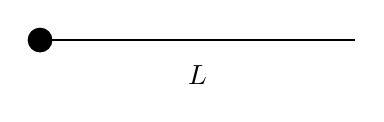
\begin{tikzpicture}[scale=1]
% Hinge
\filldraw (0,0) circle (0.15);

% Rod
\draw[thick] (0,0) -- (4,0);

\node[below] at (2,-0.2) {$L$};
\end{tikzpicture}
\end{center}

A) $0.5\%$ \\
B) $0.3\%$ \\
C) $0.6\%$ \\
D) $1\%$

\item For rolling without slipping down an incline, $a=\dfrac{g\sin\theta}{1+k}$ where $k=I/(mR^2)$. If incline angle increases by 3\% while distribution changes so that $k$ decreases by 2\%, estimate approximate fractional change in acceleration ignoring second-order terms.

% =========================
% Diagram for Question 10
% =========================
\begin{center}
\textbf{Diagram for Question 10}
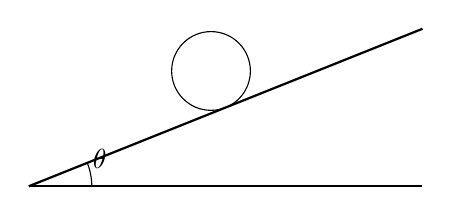
\begin{tikzpicture}[scale=1]
% Incline
\draw[thick] (0,0) -- (5,0);
\draw[thick] (0,0) -- (5,2);

% Angle
\draw (0.8,0) arc (0:{atan(2/5)}:0.8);
\node at (0.9,0.35) {$\theta$};

% Rolling object
\draw (2.5,1) ++(111.8:0.5) circle (0.5);
\end{tikzpicture}
\end{center}

A) $5\%$ \\
B) $3\%$ \\
C) $1\%$ \\
D) $0\%$

\item A rotating disc expands uniformly so that its radius increases by 2\% while mass remains constant and no external torque acts. Since $I\propto MR^2$, determine approximate fractional change in angular velocity and hence direction of change in rotational speed.

% =========================
% Diagram for Question 11
% =========================
\begin{center}
\textbf{Diagram for Question 11}
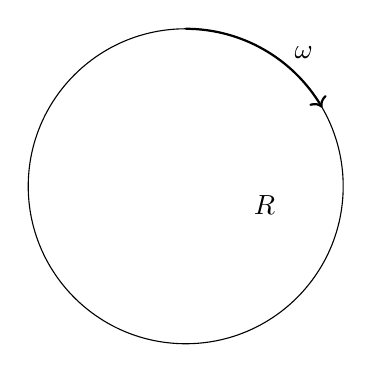
\begin{tikzpicture}[scale=1]
\draw (0,0) circle (2);
\draw[->,thick] (0,2) arc (90:30:2);
\node at (1.5,1.7) {$\omega$};
\node[below] at (1,0) {$R$};

\end{tikzpicture}
\end{center}

A) $-4\%$ \\
B) $-2\%$ \\
C) $-1\%$ \\
D) $-8\%$

\item For the same expanding disc in previous question, evaluate approximate fractional change in rotational kinetic energy after expansion, using conservation of angular momentum and neglecting higher-order small terms.

A) $0\%$ \\
B) $-4\%$ \\
C) $-8\%$ \\
D) $-2\%$

\item In a conical pendulum, $T=\dfrac{mg}{\cos\theta}$ and $\tan\theta=\dfrac{\omega^2 r}{g}$. If angular speed increases by 2\% while string length remains constant, determine approximate fractional increase in tension, neglecting second-order effects.

% =========================
% Diagram for Question 13
% =========================
\begin{center}
\textbf{Diagram for Question 13}
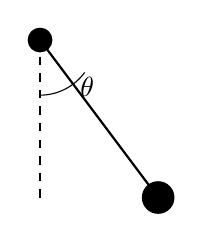
\begin{tikzpicture}[scale=1]
% Pivot
\filldraw (0,2) circle (0.15);

% String
\draw[thick] (0,2) -- (1.5,0);

% Mass
\filldraw (1.5,0) circle (0.2);

% Vertical reference
\draw[dashed] (0,2) -- (0,0);

% Angle
\draw (0,2) ++(-90:0.7) arc (-90:-36:0.7);
\node at (0.6,1.4) {$\theta$};
\end{tikzpicture}
\end{center}

A) $2\%$ \\
B) $4\%$ \\
C) $6\%$ \\
D) $8\%$

\item Orbital angular momentum of circular orbit is $L=m\sqrt{GMR}$. If orbital radius decreases by 4\% due to small impulse while motion settles into new circular orbit, determine approximate fractional change in angular momentum magnitude.

A) $-2\%$ \\
B) $-4\%$ \\
C) $-1\%$ \\
D) $-8\%$

\item A solid sphere rolls without slipping down a fixed incline. If its radius increases by 3\% while mass remains constant (density changes accordingly) and incline angle remains same, determine approximate fractional change in linear acceleration.

% =========================
% Diagram for Question 15
% =========================
\begin{center}
\textbf{Diagram for Question 15}
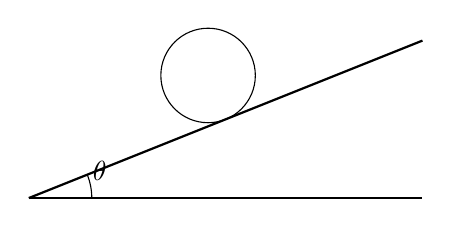
\begin{tikzpicture}[scale=1]
% Incline
\draw[thick] (0,0) -- (5,0);
\draw[thick] (0,0) -- (5,2);

% Sphere
\draw (2.5,1) ++(111.8:0.6) circle (0.6);

% Angle
\draw (0.8,0) arc (0:{atan(2/5)}:0.8);
\node at (0.9,0.35) {$\theta$};
\end{tikzpicture}
\end{center}

A) $0\%$ \\
B) $+3\%$ \\
C) $-3\%$ \\
D) $+6\%$

\end{enumerate}

\end{document}